\section*{Ejercicios}

\begin{enumerate}
\item Calcular las corrientes de malla mostradas en el circuito de la
  figura.
  
  Datos: $\; R_1 = \qty{2}{\ohm}$;\, $R_2 = \qty{5}{\ohm}$;\, $R_3 = \qty{10}{\ohm}$;\, $R_4 = \qty{4}{\ohm}$;\, $R_5 = \qty{2}{\ohm}$;\, $E_1 = \qty{25}{\volt}$;\, $E_2 = \qty{50}{\volt}$

  \begin{center}
    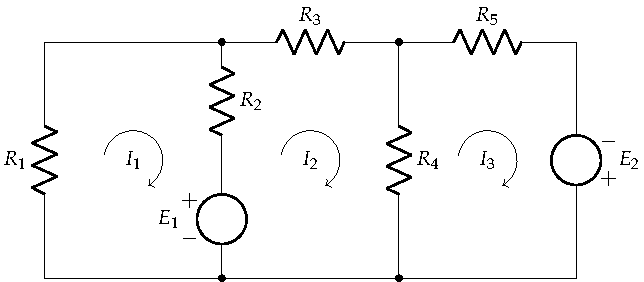
\includegraphics[height=4.2cm]{../figs/ej2_BT1.pdf}
  \end{center}

  \emph{Sol.:\; $I_1=\qty{-1.31}{\ampere};\, I_2=\qty{3.17}{\ampere};\, \qty{10.45}{\ampere}$}
	
%%%%%%%%%%%%%%%%%%%%%%%%%%%
	
\item Calcular el valor de $E$ que hace que $I_0=\qty{7.5}{\milli\ampere}$ en el
  circuito de la figura.

  Datos: $\; R_1 = \qty{8}{\ohm}$;\, $R_2 = \qty{7}{\ohm}$;\, $R_3 = \qty{4}{\ohm}$;\, $R_4 = \qty{6}{\ohm}$;\, $R_5 = \qty{6}{\ohm}$;\, $R_6 = \qty{12}{\ohm}$ 
  
  \begin{center}
    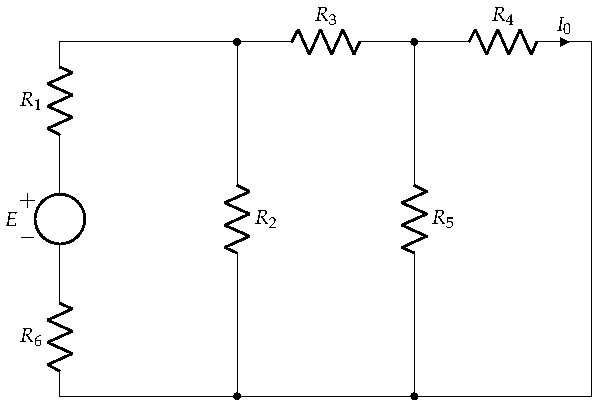
\includegraphics[height=5.5cm]{../figs/ej3_BT1.pdf}
  \end{center}
  
  \emph{Sol.:\; $U_s=\qty{0.705}{\volt}$}
	
%%%%%%%%%%%%%%%%%%%%%%%%%%%
	
\item Calcular la intensidad $I$ en el circuito de la figura.

    Datos: $\; R_1 = \qty{27}{\ohm}$;\, $R_2 = \qty{47}{\ohm}$;\, $R_3 = \qty{27}{\ohm}$;\, $E_1 = \qty{460}{\volt}$;\, $E_2 = \qty{200}{\volt}$
    
  \begin{center}
    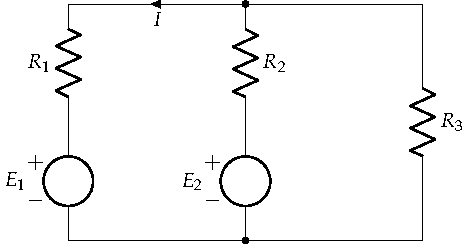
\includegraphics{../figs/ej4_BT1.pdf}
  \end{center}

  \emph{Sol.:\; $I=\qty{-8.77}{\ampere}$}

%%%%%%%%%%%%%%%%%%%%%%%%%%%
		
\item En el circuito de la figura obtener las intensidades de
  corriente señaladas primero mediante un análisis por el método de
  las mallas y posteriormente mediante un análisis por el método de
  los nudos.

  Datos: $\; R_1 = \qty{2}{\ohm}$; $R_2 = \qty{1}{\ohm}$; $R_3 = \qty{4}{\ohm}$; $R_4 = \qty{5}{\ohm}$; $R_5 = \qty{3}{\ohm}$; $E_1 = \qty{10}{\volt}$; $E_2 = \qty{6}{\volt}$
  
  \begin{center}
    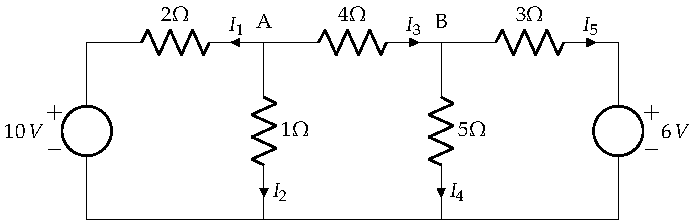
\includegraphics{../figs/ej8_BT1.pdf}
  \end{center}

  \emph{Sol.:\;
    $I_1=\qty{-3.31}{\ampere};\, I_2=\qty{3.37}{\ampere};\, I_3=\qty{-0.06}{\ampere};\, 
    I_4=\qty{0.73}{\ampere};\,  I_5=\qty{-0.79}{\ampere};\, $}
 	
%%%%%%%%%%%%%%%%%%%%%%%%%%%

\item Analizar el circuito de la figura mediante el método de las mallas, obteniendo la corriente de cada una de las ramas. Con este resultado, calcular la diferencia de potencial entre A y B, y realizar un balance de potencias comparando la potencia de los elementos activos y la de los elementos pasivos. 

Datos: $\; R_1 = R_2 = \qty{1}{\ohm};\, R_3 = \qty{2}{\ohm};\, R_4 = \qty{3}{\ohm};\, R_5=\qty{4}{\ohm};\, \epsilon_1=\qty{118}{\volt};\, \epsilon_2 = \qty{236}{\volt};\, \epsilon_3 = \qty{118}{\volt}$\\

  \begin{center}
    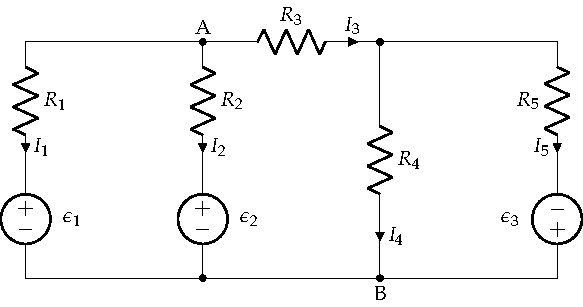
\includegraphics{../figs/mallas2.pdf}
  \end{center}

 \emph{Sol.:\;
    $I_1 = \qty{32}{\ampere};\, I_2 = \qty{-86}{\ampere};\, I_3 =\qty{54}{\ampere};\, I_4 = \qty{14}{\ampere};\, I_5 = \qty{40}{\ampere};\,
    U_{AB}=\qty{150}{\volt};\, P_g = P_R$}
 	
%%%%%%%%%%%%%%%%%%%%%%%%%%%

\item En el circuito de la figura, determinar:
  \begin{itemize}
  \item Todas las intensidades de rama señaladas
  \item Carga, polaridad y energía almacenada en los condensadores
  \item Balance de potencias
  \end{itemize}
    Datos: $\; R_i = \qty[parse-numbers=false]{i}{\ohm}$;\, $C_i = \qty[parse-numbers=false]{i}{\micro\farad}$;\, $E_1 = \qty{8}{\volt}$;\, $E_2 = \qty{6}{\volt}$;\, $E_3 = \qty{4}{\volt}$

  \begin{center}
    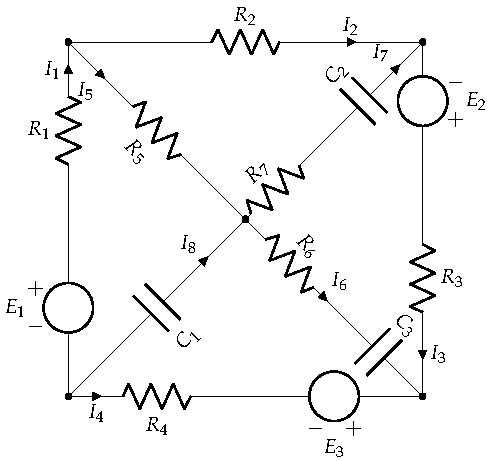
\includegraphics[height=7.2cm]{../figs/ej9_BT1.pdf}
  \end{center}

  \emph{Sol.:\;
    $I_1=I_2=I_3=-I_4=\qty{1}{\ampere};\,  I_5=I_6=I_7=\qty{0}{\ampere};\, Q_{1\si{\micro\farad}}=\qty{-7}{\micro\coulomb};\, Q_{2\si{\micro\farad}}=\qty{-4}{\micro\coulomb};\, Q_{3\si{\micro\farad}}=\qty{3}{\micro\coulomb};\, E_{1\si{\micro\farad}}=\qty{24.5}{\micro\joule};\, E_{2\si{\micro\farad}}=\qty{4}{\micro\joule};\, E_{3\si{\micro\farad}}=\qty{1.5}{\micro\joule}$}

%%%%%%%%%%%%%%%%%%%%%%%%%%%

\item Aplicar el método de los nudos en el circuito de la figura para
  determinar:
  \begin{itemize}
  \item Los potenciales de los nudos A, B, C y D.
  \item Las intensidades de corriente señaladas.
  \item Carga, polaridad y energía almacenada en los condensadores,
    supuestos sin carga inicial.
  \end{itemize}
  Datos:
  $\; R_i = \mathrm{i\ } \Omega;\, C_i = \mathrm{i\ } \si{\micro\farad};\, E_1 = \qty{6}{\volt};\, E_2
  = \qty{18}{\volt};\, E_3 = \qty{6}{\volt}$
  \begin{center}
    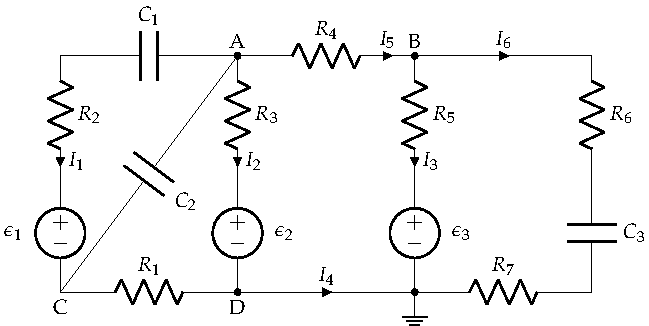
\includegraphics[]{../figs/nudos_condensadores.pdf}
  \end{center}

  \emph{Sol.:\;
    $U_A=\qty{15}{\volt};\, U_B=\qty{11}{\volt};\, U_C=U_D=\qty{0}{\volt};\, I_1=I_6=\qty{0}{\ampere};\, I_2=I_4=\qty{-1}{\ampere};\, I_3=I_5=\qty{1}{\ampere};\,
    q_1=\qty{9}{\micro\coulomb};\, q_2=\qty{30}{\micro\coulomb};\, q_3=\qty{33}{\micro\coulomb};\, E_{C1}=\qty{40.5}{\micro\joule};\,
    E_{C2}=\qty{225}{\micro\joule};\, E_{C2}=\qty{181.5}{\micro\joule}$}

%%%%%%%%%%%%%%%%%%%%%%%%%%%

\item En el circuito de la figura, donde se sabe
  que la carga inicial de los condensadores era de
  $\qty{10}{\micro\coulomb}$ para $C_1$ y de
  $\qty{20}{\micro\coulomb}$ para $C_2$ con las polaridades indicadas,
  se pide determinar:
  \begin{itemize}
  \item Intensidades de corriente señaladas
  \item Potenciales en los puntos A, B, C, D, E y F
  \end{itemize}

  Datos:
  $\;\epsilon_1=\SI{90}{\volt};\, \epsilon_2=\SI{60}{\volt};\,
  \epsilon_3=\SI{30}{\volt};\, R_{1}= R_2 = R_3 =
  \SI{10}{\ohm};\, R_{4}= R_5 = \SI{30}{\ohm};\, C_{1}=
  \SI{10}{\micro\farad};\, C_{2}= \SI{20}{\micro\farad};\, L_1 =
  \SI{1}{\micro\henry}$

  \begin{center}
    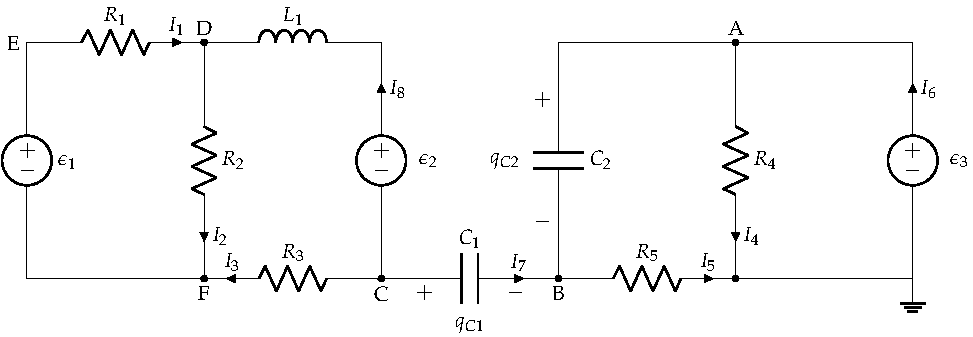
\includegraphics[scale = 0.9]{../figs/mallas_carga_inicial.pdf}
  \end{center}

\emph{Sol.:\;
  $I_1=\qty{4}{\ampere};\, I_2=\qty{5}{\ampere};\, I_3=\qty{-1}{\ampere};\, I_4=I_6=\qty{1}{\ampere};\, I_5=I_7=\qty{0}{\ampere};\, I_8=\qty{1}{\ampere};\, U_A=\qty{30}{\volt};\, U_B=\qty{0}{\volt};\,
  U_C=\qty{1}{\volt};\, U_D=\qty{61}{\volt};\, U_E=\qty{101}{\volt};\, U_F=\qty{11}{\volt};\,$}

%%%%%%%%%%%%%%%%%%%%%%%%%%%

\item En el circuito de la figura, los condensadores se conectaron sin
  carga. Mediante el método de las mallas, se debe determinar:
  \begin{itemize}
  \item Intensidades de corriente señaladas
  \item Potenciales en los puntos A, B, C y D
  \item Polaridades, cargas, y energías de los condensadores
  \item Balance de potencias
  \end{itemize}
  Datos:
  $\; \epsilon_{1}=\qty{118}{\volt};\, \epsilon_{2}=\qty{236}{\volt};\, \epsilon_{3}=\qty{118}{\volt};\,
  R_{1}= \qty{4}{\ohm};\, R_{2}=R_{3}=\qty{1}{\ohm};\, R_{4}= \qty{3}{\ohm};\,
  R_{5}=\qty{2}{\ohm};\, C_{1}=C_{2}=C_{3}=\qty{2}{\micro\farad};\, L_1 = L_2 = L_3 = \qty{1}{\milli\henry}$
  \begin{center}
    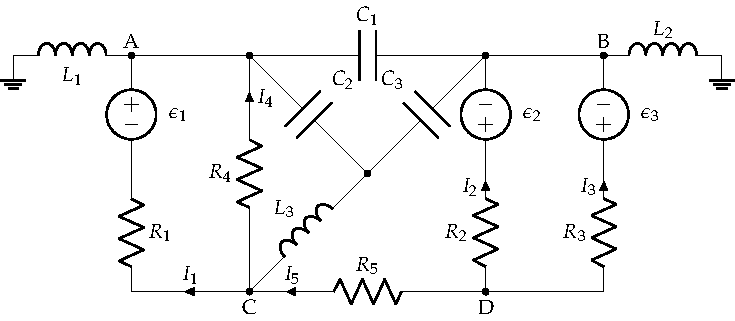
\includegraphics{../figs/mallas_condensadores.pdf}
  \end{center}

  \emph{Sol.:\;
    $I_1=\qty{40}{\ampere};\, I_2=\qty{-86}{\ampere};\, I_3=\qty{32}{\ampere};\, I_4=\qty{14}{\ampere};\, I_5=\qty{54}{\ampere};\, U_A=U_B=\qty{0}{\volt};\,
    U_C=\qty{42}{\volt};\, U_D=\qty{150}{\volt};\, U_{C1}=\qty{0}{\volt};\, q_1=\qty{0}{\coulomb};\, E_{C1}=\qty{0}{\joule};\, U_{C2}=\qty{-42}{\volt};\,
    q_2=\qty{84}{\micro\coulomb};\, E_{C2}=\qty{1.76}{\milli\joule};\, U_{C3}=\qty{-42}{\volt};\, q_3=\qty{84}{\micro\coulomb};\, E_{C3}=\qty{1.76}{\milli\joule};\, P_g = P_R$}

%%%%%%%%%%%%%%%%%%%%%%%%%%%

\item En el circuito de la figura, se debe determinar:
  \begin{itemize}
  \item Las ecuaciones para el cálculo de las intensidades
  \item Todas las intensidades indicadas
  \item Potenciales en todos los nudos
  \item Carga y energía almacenada en los condensadores
  \end{itemize}

  Datos: $\; R_1 = \qty{2}{\ohm}$;\, $R_2 = \qty{4}{\ohm}$;\, $R_3 = \qty{2}{\ohm}$;\, $R_4 = \qty{1}{\ohm}$;\, $R_5 = \qty{2}{\ohm}$;\, $R_6 = \qty{1}{\ohm}$;\, $E_1 = \qty{8}{\volt}$;\, $E_2 = \qty{8}{\volt}$;\, $C_i = \qty[parse-numbers=false]{i}{\micro\farad}$
  
  \begin{center}
    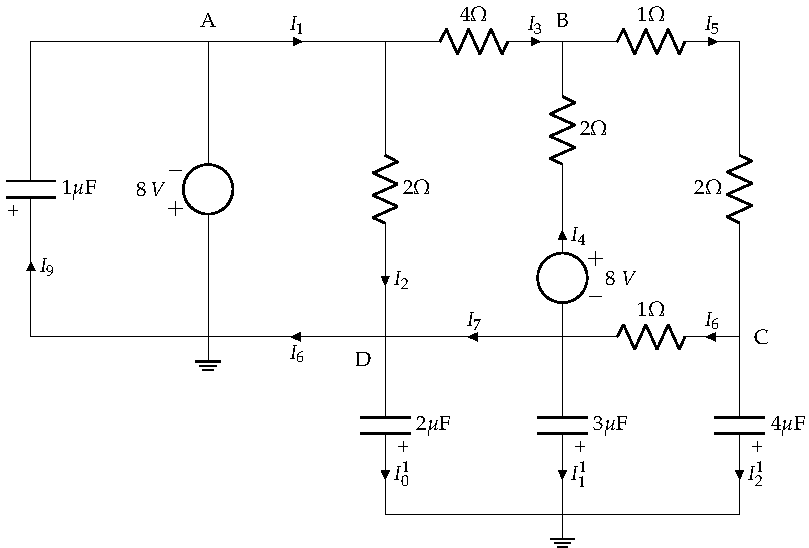
\includegraphics[height=8cm]{../figs/ej11_BT1.pdf}
  \end{center}

  \emph{Sol.:\;
    $I_1=I_8=\qty{-6.5}{\ampere};\, I_2=\qty{-4}{\ampere};\, I_3=I_7=\qty{-2.5}{\ampere};\, I_4=\qty{3}{\ampere};\, I_5=I_6=\qty{0.5}{\ampere};\, U_A=\qty{-8}{\volt};\,
    U_B=\qty{2}{\volt};\, U_C=\qty{0.5}{\volt};\, U_D=\qty{0}{\volt};\, Q_{1\si{\micro\farad}}=\qty{8}{\micro\coulomb};\, Q_{2\si{\micro\farad}}=Q_{3\si{\micro\farad}}=\qty{0}{\micro\coulomb};\, Q_{4\si{\micro\farad}}=\qty{-2}{\micro\coulomb};\, E_{1\si{\micro\farad}}=\qty{32}{\micro\joule};\, E_{2\si{\micro\farad}}=E_{3\si{\micro\farad}}=\qty{0}{\joule};\, E_{4\si{\micro\farad}}=\qty{0.5}{\micro\joule}$}

\newpage

%%%%%%%%%%%%%%%%%%%%%%%%%%%

\item En el circuito de la figura, se debe determinar:
  \begin{itemize}
  \item Las corrientes señaladas.
  \item El balance de potencias, diferenciando entre elementos activos
    y elementos pasivos.
  \item Los potenciales en los puntos A, B y C.
  \item La carga y polaridad en los condensadores, supuestos sin carga
    inicial.
  \end{itemize}
  Datos:
  $\; \epsilon_1 =\qty{1}{\volt};\, \epsilon_2 =\qty{7}{\volt};\, R_i = \qty{1}{\ohm};\, C_i = i\, \si{\micro \farad}$

  \begin{center}
    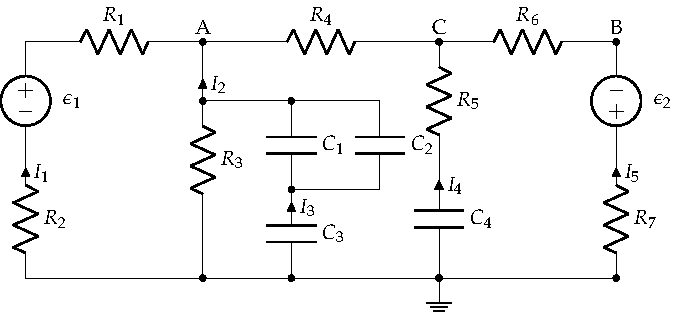
\includegraphics[height=5cm]{../figs/mallas_agrupacion_condensadores.pdf}
  \end{center}

  \emph{Sol.:\;
    $I_1=I_2=\qty{1}{\ampere};\, I_3=I_4=\qty{0}{\ampere};\, I_5=\qty{-2}{\ampere};\, \sum_\epsilon P_\epsilon = \sum_R P_R;\, U_A=\qty{-1}{\volt};\, U_B=\qty{-5}{\volt};\, U_C=\qty{-3}{\volt};\, q_1=\qty{0.5}{\micro\coulomb};\, q_2 = \qty{1}{\micro\coulomb};\, q_3=\qty{1.5}{\micro\coulomb};\, q_4=\qty{12}{\micro\coulomb}$}

%%%%%%%%%%%%%%%%%%%%%%%%%%%

\item El circuito de la figura está funcionando en régimen
  estacionario. Los condensadores estaban inicialmente
  descargados. Resuelve el circuito mediante el método que consideres
  conveniente para obtener los siguientes resultados:
  \begin{itemize}
  \item Las intensidades señaladas.
  \item Polaridad y energía almacenada en los condensadores.
  \item Balance de potencias.
  \end{itemize}
  Datos:
  $\; \epsilon_{1}=\qty{40}{\volt};\, \epsilon_{2}=\qty{22}{\volt};\, \epsilon_{3}=\qty{20}{\volt};\,
  C_{1}=C_{2}=C_{3}=\qty{2}{\micro\farad};\, R_{g1}=R_{g2}=R_{g3}=\qty{4}{\ohm};\,
  R_{1}=R_{2}=R_{3}=R_{4}=\qty{2}{\ohm};\, R_{5}=R_{6}=R_{7}=\qty{1}{\ohm}$
  \begin{center}
    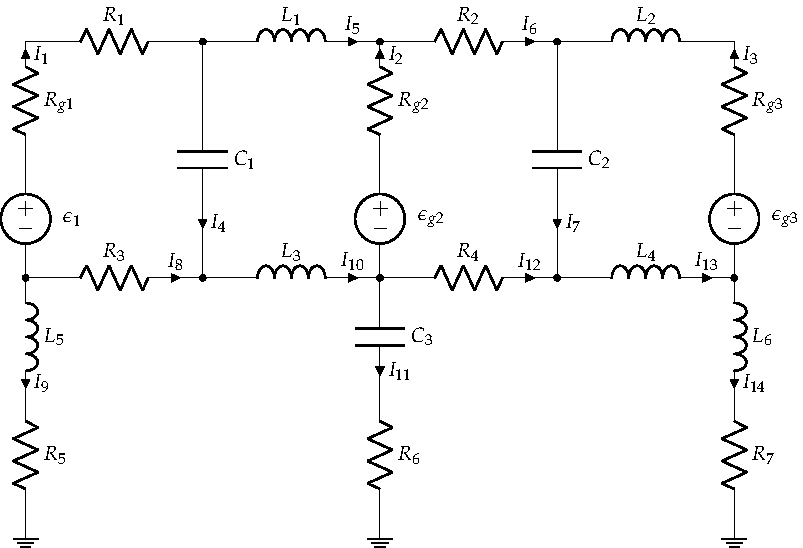
\includegraphics[height=8cm]{../figs/mallas_condensadores_bobinas.pdf}
  \end{center}
  \emph{Sol.:\;
    $I_1=I_5=\qty{2}{\ampere};\, I_2=I_3=I_8=I_{10}=\qty{-1}{\ampere};\,
    I_4=I_7=I_{11}=I_{12}=I_{13}=\qty{0}{\ampere};\, I_6=I_{14}=\qty{1}{\ampere};\, E_{C1}=\qty{0.676}{\milli\joule};\,
    E_{C2}=\qty{0.576}{\milli\joule}; \, E_{C3}=\qty{1}{\micro\joule}; P_g = P_R$}
 
%%%%%%%%%%%%%%%%%%%%%%%%%%%

\item En el circuito de la figura, obtener las
  intensidades de corriente señaladas mediante un análisis por el
  método de las mallas y mediante un análisis por el método de los
  nudos.

  Datos: $\; R_1 = \qty{9}{\ohm}$; $R_2 = \qty{4}{\ohm}$; $R_3 = \qty{18}{\ohm}$; $R_4 = R_5 = R_6 = \qty{20}{\ohm}$; $E_1 = \qty{16}{\volt}$; $I_g = \qty{2}{\ampere}$
  
  \begin{center}
    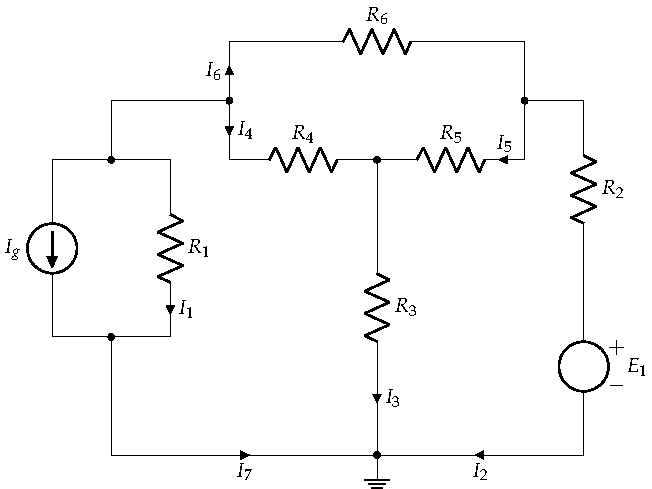
\includegraphics{../figs/ej12_BT1.pdf}
  \end{center}

  \emph{Sol.:\;
    $I_1=\qty{-0.74}{\ampere};\,I_2=\qty{-1.33}{\ampere};\,I_3=\qty{0.07}{\ampere};\,I_4=\qty{-0.39}{\ampere};\,I_5=\qty{0.46}{\ampere};\,I_6=\qty{-0.87}{\ampere};\,I_7=\qty{1.26}{\ampere}$}

%%%%%%%%%%%%%%%%%%%%%%%%%%%

\item Resolver el circuito por el método que se estime conveniente, obteniendo:
    \begin{itemize}
        \item El valor de las corrientes indicadas ($I_1, I_2, I_3, I_4, I_5$).
        
        \item La carga y polaridad de $C_1, C_2$ y $C_3$.

        \item La potencia entregada o absorbida por los elementos activos.
    \end{itemize}
    
    \begin{minipage}{0.65\linewidth}
      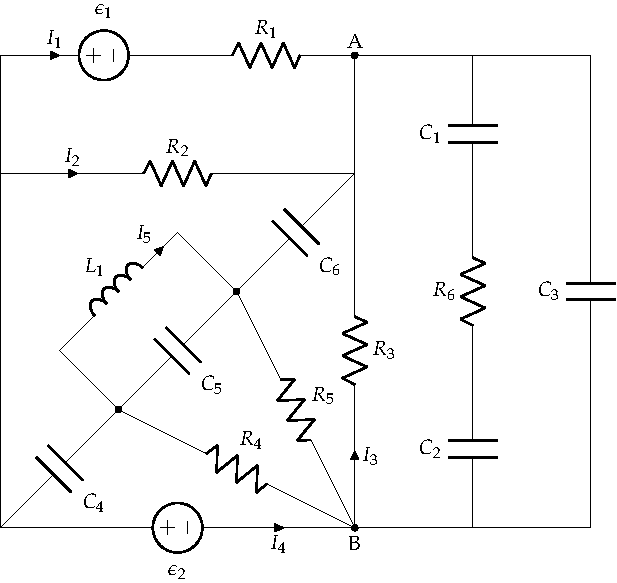
\includegraphics[scale=0.9]{figs/BT1_ej14_enunciado.pdf}
    \end{minipage}
    \begin{minipage}{0.35\linewidth}
    
        \hspace{5mm}Datos:
    
        \vspace{2mm}    
        \hspace{5mm}$R_1 = R_2 = \qty{2}{\ohm}$
    
        \vspace{1mm}
        \hspace{5mm}$R_3 = R_4 = R_5 = R_6 = \qty{1}{\ohm}$
    
        \vspace{1mm}
        \hspace{5mm}$C_i = i\,\si{\micro\farad}$
    
        \vspace{1mm}
        \hspace{5mm}$L_1 = 1\,\si{\milli\henry}$
    
        \vspace{1mm}
        \hspace{5mm}$\epsilon_1 = \qty{10}{\volt}$
    
        \vspace{1mm}
        \hspace{5mm}$\epsilon_2 = \qty{10}{\volt}$
        
    \end{minipage}

    \emph{Sol.:\; $I_1=\qty{-1.25}{\ampere};\; I_2=\qty{3.75}{\ampere};\; I_3=I_4=\qty{-2.5}{\ampere};\; I_5=\qty{0}{\ampere};\; q_1 = q_2 = \dfrac{5}{3}\,\si{\micro\coulomb};\; q_3 = \qty{7.5}{\micro\coulomb};\; P_{\epsilon1} = \qty{12.5}{\watt};\; P_{\epsilon2} = \qty{25}{\watt}$}

%%%%%%%%%%%%%%%%%%%%%%%%%%%

\item Calcular la intensidad que circula por la resistencia de 30$\,\Omega$ del circuito de la figura aplicando el principio de
  superposición.

  Datos: $\; R_1 = \qty{20}{\ohm}$; $R_2 = \qty{30}{\ohm}$; $R_3 = \qty{20}{\ohm}$; $E_1 = \qty{32}{\volt}$; $E_2 = \qty{64}{\volt}$; $I_g = \qty{4}{\ampere}$
  
  \vspace{-2mm}
  \begin{center}
    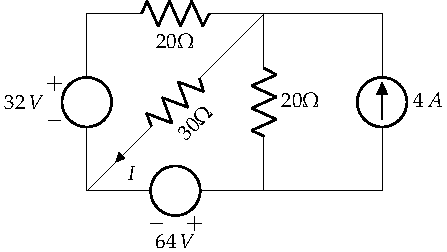
\includegraphics[height=4cm]{../figs/ej16_BT1.pdf}
  \end{center}  

  \vspace{-6mm}
  \emph{Sol.:\; $I=\qty{2.2}{\ampere}$}

%%%%%%%%%%%%%%%%%%%%%%%%%%%

\item Obtener el generador equivalente de Thévenin del circuito de la
  figura respecto de A y B. A partir de este generador, calcula la
  resistencia a colocar en A-B para obtener la máxima potencia,
  calculando esta potencia y la potencia entregada por el generador
  $\epsilon$.

  Datos:
  $\; \epsilon = \qty{54}{\volt};\; R_1 = R_4 = \qty{8}{\ohm};\;
  R_2 = R_3 = \qty{10}{\ohm}$

    \vspace{-1mm}
  \begin{center}
    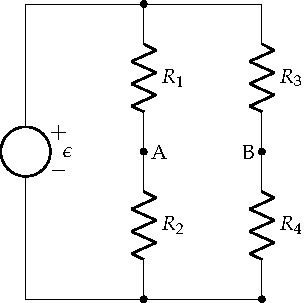
\includegraphics[height=4.75cm]{../figs/Thevenin2}
  \end{center}

    \vspace{-2mm}
    \emph{Sol.:\;
      $R_{AB} = \dfrac{80}{9}\,\si{\ohm}; \; P_R = \qty{1.0125}{\watt}; \;
      P_\epsilon = \qty{2.025}{\watt}$}

%%%%%%%%%%%%%%%%%%%%%%%%%%%

  \item Determinar el equivalente Thévenin del circuito de la figura
    entre los nudos A-B. ¿Qué resistencia habría que conectar en
    dichos terminales para transferir la máxima potencia? ¿Cuál sería
    dicha potencia?

    Datos: $\; R_1 = R_2 = \qty{4}{\ohm}$;\; $R_3 = \qty{2}{\ohm}$;\; $E = \qty{10}{\volt}$;\; $I_g = \qty{8}{\ampere}$

    \vspace{-3mm}
    \begin{center}
      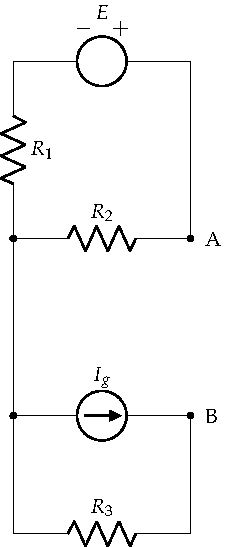
\includegraphics[height=9cm]{../figs/ej17_BT1.pdf}
    \end{center}

    \emph{Sol.:\;
      $\epsilon_{th}=5-16=\qty{-11}{\volt};\; R_{th}=\qty{4}{\ohm};\;
      R_L=\qty{4}{\ohm};\;P_{max}=\qty{7.56}{\watt}$}

%%%%%%%%%%%%%%%%%%%%%%%%%%%

  \item Obtener el generador equivalente de Thévenin del circuito de la figura respecto de A y B.
  
    Datos: $\; I_g=\qty{10}{\ampere};\; R_1=\qty{1}{\ohm};\; \alpha=5$
    \begin{center}
      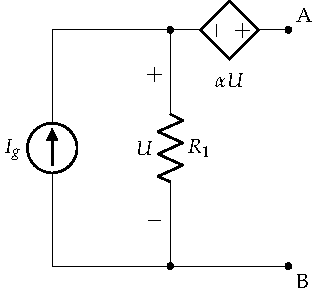
\includegraphics[height=4.75cm]{../figs/Thevenin1.pdf}
    \end{center}

    \emph{Sol.:\; $\epsilon_{th}=\qty{60}{\volt};\; R_{th}=\qty{62}{\ohm}$}

%%%%%%%%%%%%%%%%%%%%%%%%%%%

    \item En el circuito de la figura, se debe calcular el equivalente de Norton entre terminales A-B.

    \begin{minipage}{0.6\linewidth}
      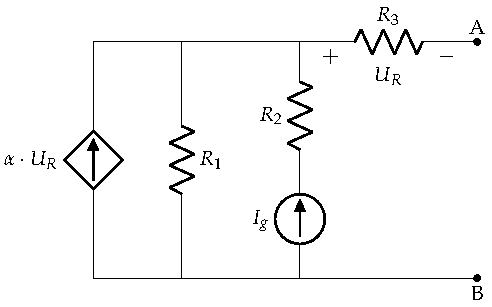
\includegraphics[height=4.75cm]{figs/BT1_ej19_enunciado.pdf}
    \end{minipage}
    \begin{minipage}{0.4\linewidth}
      Datos:
      \vspace{2mm}
      
      $R_1 = R_3 = \qty{1}{\ohm}$\\[1mm]
      $R_2 = \qty{2}{\ohm}$\\[1mm]
      $\alpha = 0.5\,\si{\ohm}^{-1}$\\[1mm]
      $I_g = \qty{6}{\ampere}$
    \end{minipage}

    \emph{Sol.:\; 
      $I_N = \qty{4}{\ampere};\; R_N = \dfrac{3}{2}\,\si{\ohm}$}
      
%%%%%%%%%%%%%%%%%%%%%%%%%%%

  \item En el circuito de la figura, calcular:
    \begin{itemize}
    \item La corriente del generador equivalente de Norton respecto de
      A y B, $I_N$.
    \item La resistencia del generador equivalente de Norton respecto
      de A y B, $R_N$.
    \item La resistencia de carga que se debe conectar entre A y B
      para conseguir la máxima potencia disponible, y el valor de esta
      potencia.
    \end{itemize}
    Datos:
    $\; R = \qty{1}{\ohm};\; \epsilon_g = \qty{10}{\volt};\; \alpha = \qty{2}{\ohm};\; \beta = 1$

    \begin{center}
      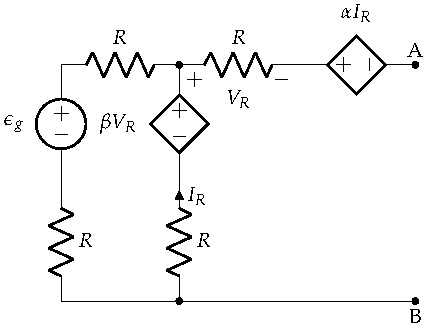
\includegraphics[height=5.5cm]{../figs/norton.pdf}
    \end{center}

\emph{Sol.:\;
  $I_N=\dfrac{10}{3}\,\si{\ampere};\; R_N=\qty{3}{\ohm};\; R_L=\qty{3}{\ohm};\;
  P_L=\dfrac{25}{3}\,\si{\watt}$}

\end{enumerate}

%%% Local Variables:
%%% mode: latex
%%% TeX-master: "enunciados_ejercicios_TC"
%%% ispell-local-dictionary: "castellano"
%%% End:
